\subsection{Components' Structure}
The presented Component Diagram has the aim to show in a more precise and detailed way which components are in each layer and how they interact.\\
To be more precise in the left it is possible to see the presentation layer devided in three components:
\begin{itemize}
	\item \textbf {User's Mobile App:} it is the user's application via device; that is the only possible interface for a user and it is 			formed by a \textit {Data Collector} and a \textit {Data Processor} components which have the aim to collect data from the 			external device containing all the necessary sensors to gather health parameters of every user ; a \textit {GPS Manager} 			which interfaces directly with the device's GPS needed in case of health parameter under the threshold (see RASD for 				more details); a \textit {GUI Manager} which is foundational to handle all actions made by users and a \textit {Controller} 			which is the bridge between the client's components and the application layer.
	\item \textbf {Third party's Mobile App:} it is the third party's application via device. This particular stakeholder doesn't need 			any GPS or Data manager because the aim of its app is to obtain data  of a single user or of a group of users, that's the 			reason why it is just formed by a \textit{ GUI Manager} and a \textit {Controller}. The aim of those two elements is the same 			presented for the user's mobile app.
	\item \textbf {Third Party's Web App:} the different aim of the app related to this stakeholder implies the necessity of a 			desktop application which is dial by the same components of the Mobile one.
\end{itemize}The application layer is also formed by three different components:
\begin{itemize}
	\item \textbf{Application Logic:} it contains the whole logic and algorithms which stay under the application and make it runs in 			a proper way. This component will be better analyzed in a dedicayìted subsection in which all its services will be presented into 			a class diagram. 
	\item \textbf{ ASOS Manager:} this component is in charge of interfacing with the external emergency service in case the 			related algorithms finds out that the user is an unhealthy one.
	\item \textbf{Data Persistence Unit:} it has a constant connection to the data layer and it has the aim to handle all possible 			dynamic behaviors related to operations on data.
\end{itemize}
\begin{figure}[h!]
	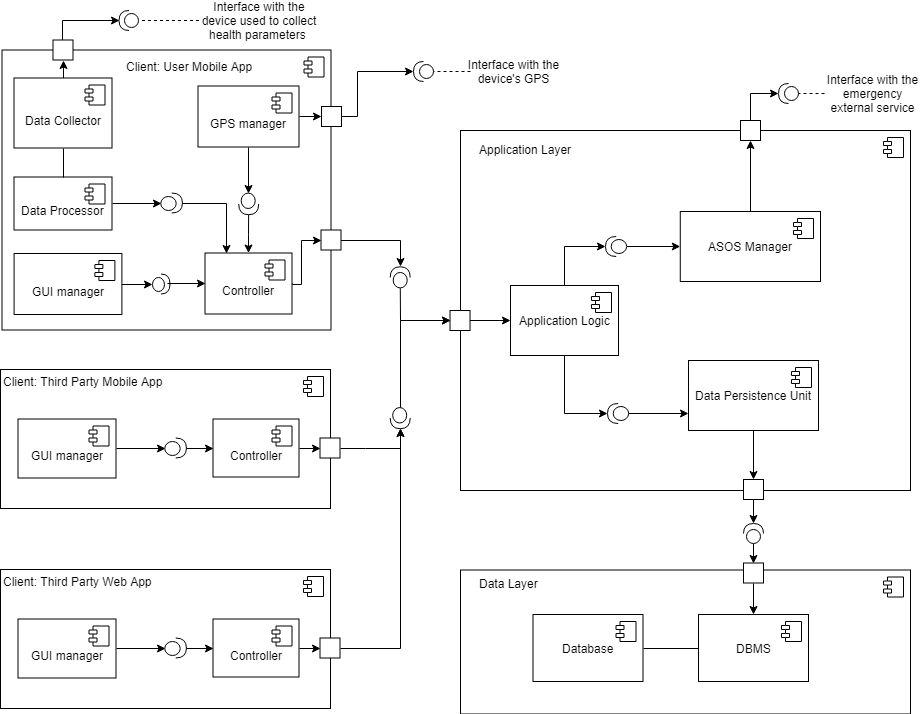
\includegraphics[width=1.0\textwidth]{./pictures/component_diagram.png}\par
	\caption{Component diagram}
\end{figure}
\FloatBarrier

\subsection{Application Logic}
To better describe the model's and controller's structure, is presented an UML class diagram more precise than the one in the RASD document. \\

\begin{figure}[h!]
	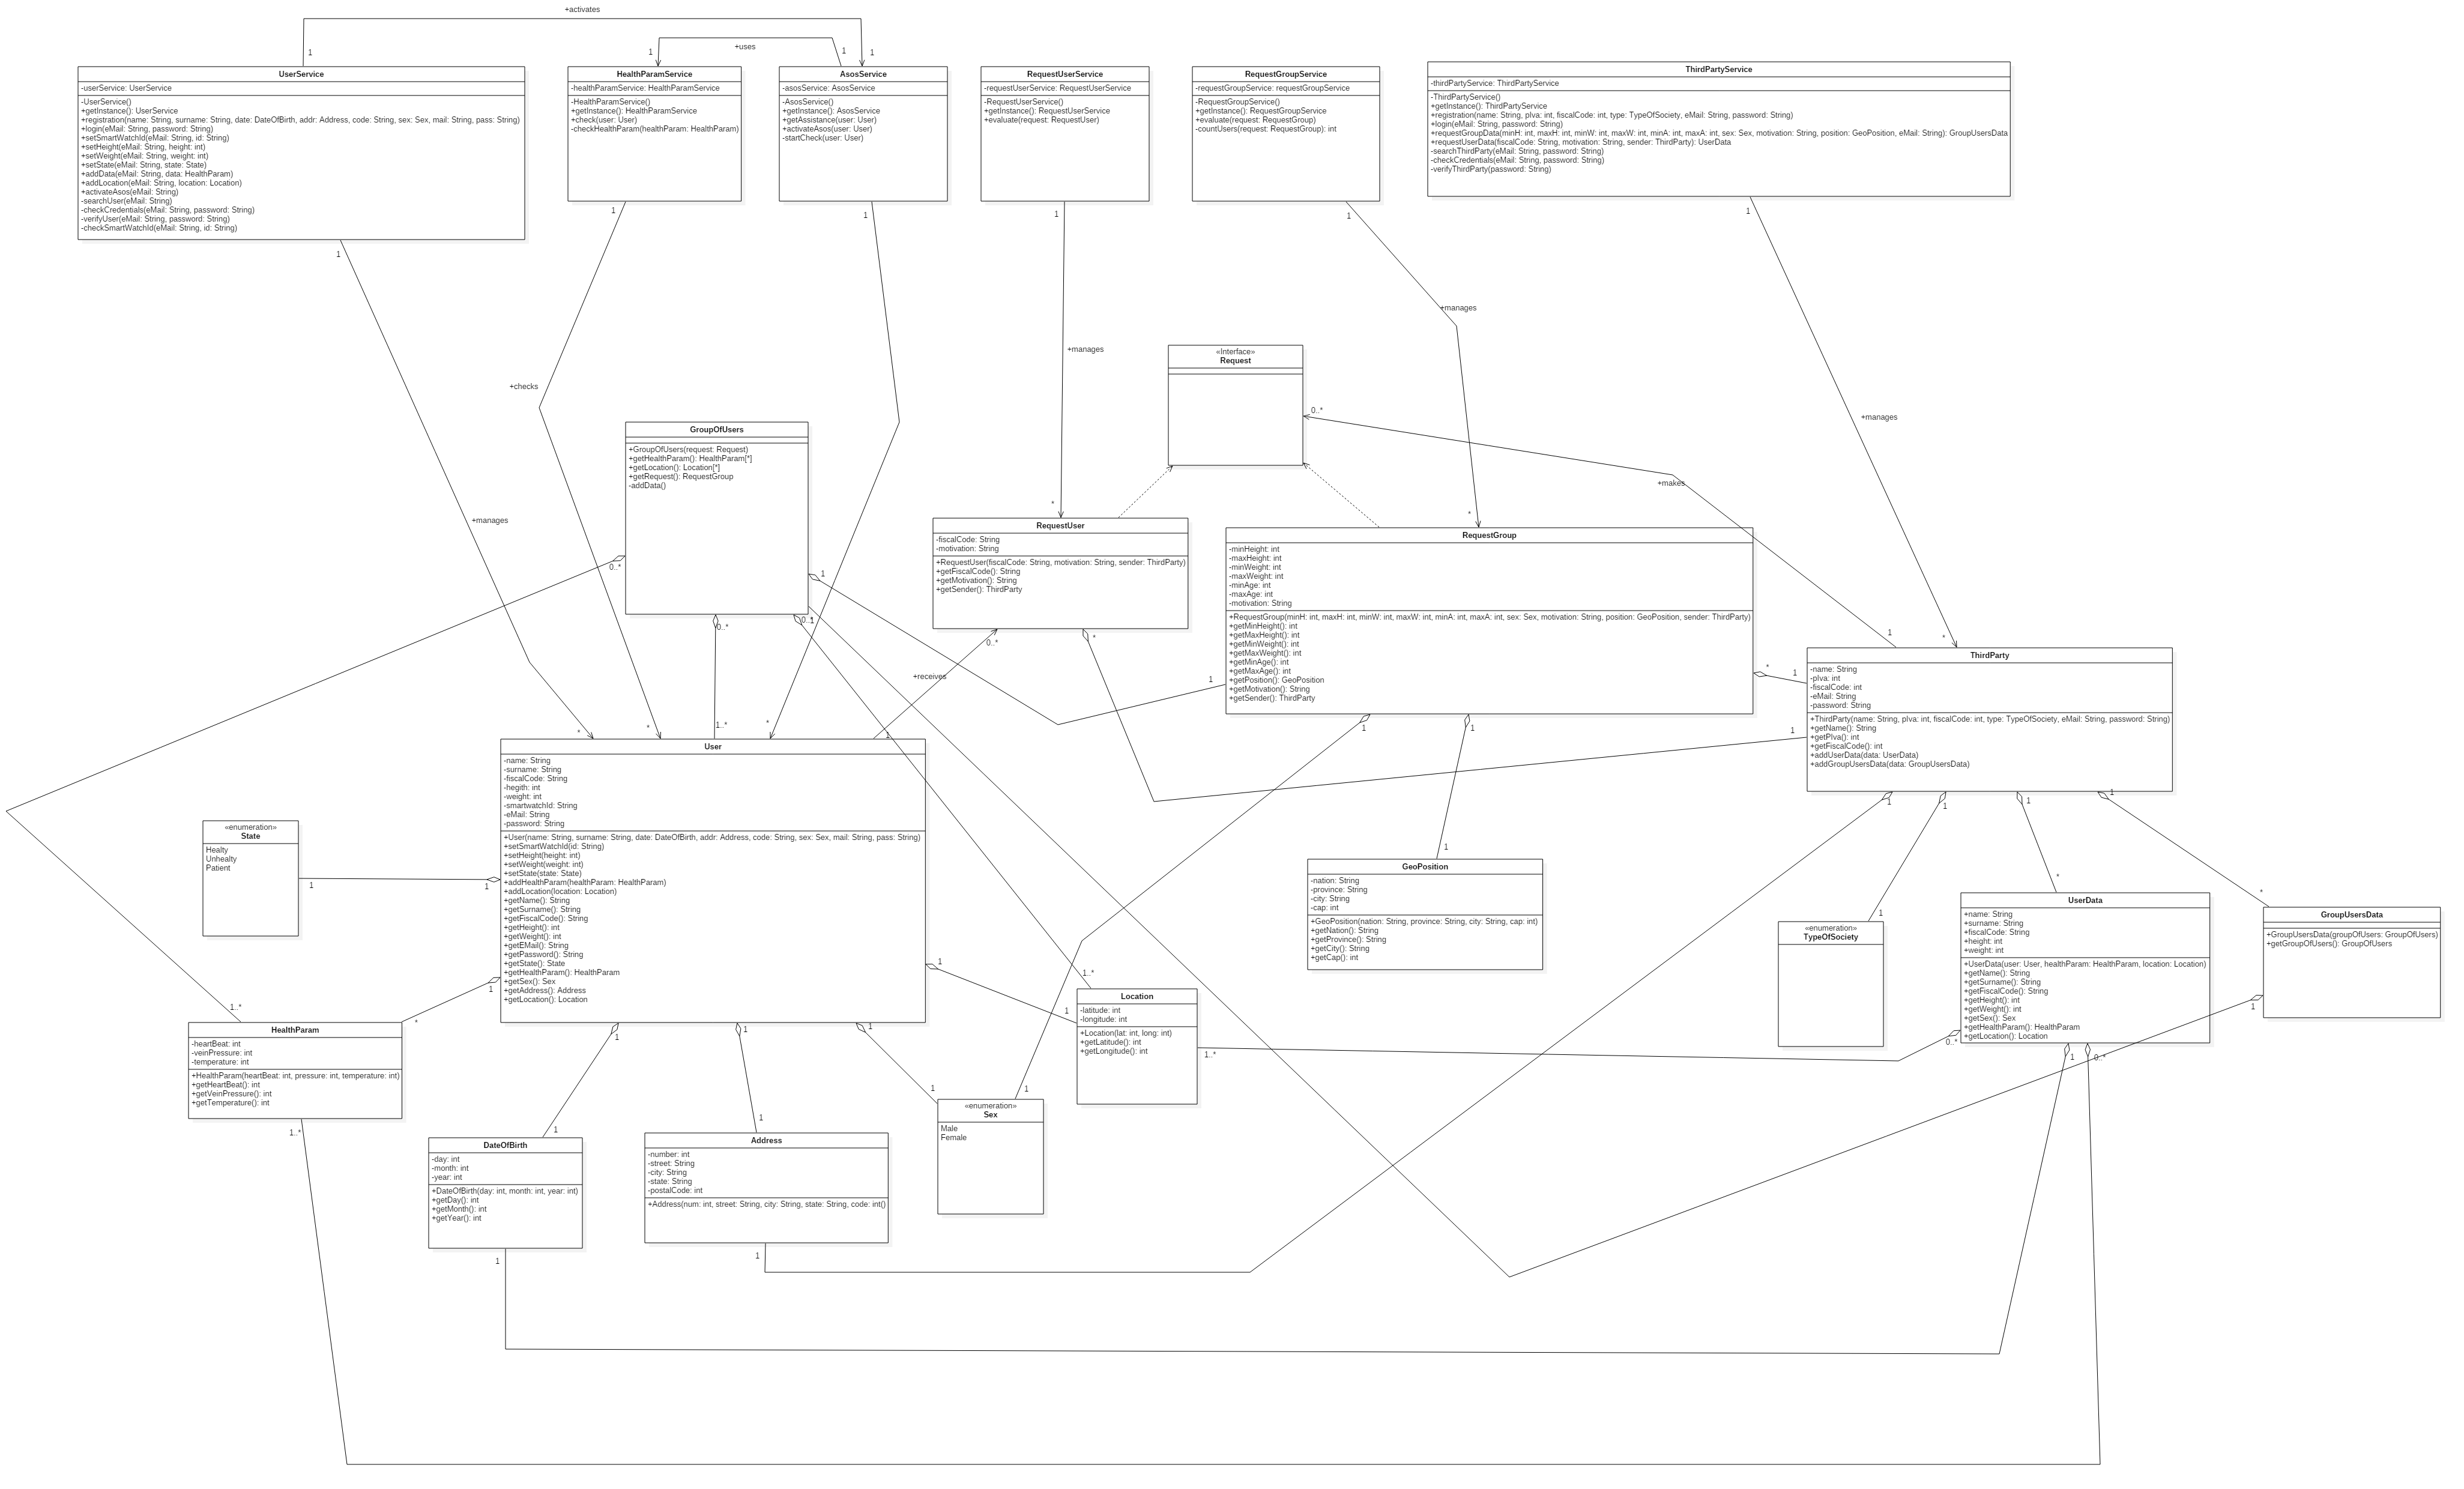
\includegraphics[width=1.0\textwidth]{./pictures/class_diagram.png}\par
	\caption{Class diagram showing the model of the appliation, it also contains all manager classes which have the aim to handle 			all possible dynamic actions.}
\end{figure}
\FloatBarrier
Note that the presented class diagram is intended as a guide for the implementation and integration of the model's part of the software.


\subsection{Database}
The data layer must contain the DB and also a DBMS component necessary to manage all possible operation, such as insertion, deletion, update, that can be done on data inside the storage unit. The chosen DBMS must guarantee the correct working of transaction according to the ACID properties.\\
A RDBMS is the best choice for this app because it adheres to the ACID properties; guarantees high performances by using indexis to sort data and by supporting both desktop and web apps and also guarantees data security providing a layer of protection for sensitive data. Using a RDBMS it is also possible to build  the DB structure and clearly define the relations between data.\\ 
As said in the previous section, the chosen architecture is composed by closed layers and for this reason  the data layer, the one which contains the stored data, can only be accessed by the Application's one, via a dedicated interface. Bacause of this it is necessary to provide a persistence unit which can handle all possible behaviors. Credentials and sensible data as personal informations must be encripted to avoid any possible privacy violation.\\
The Entity Relational diagram in figure describe a first relational model of the Database. The rectangual shapes represent the entities; the circles all possible attributes related to an entity in particular all cirles filled in black are the entities key and the relationships are represented by diamonds.

\begin{figure}[h!]
	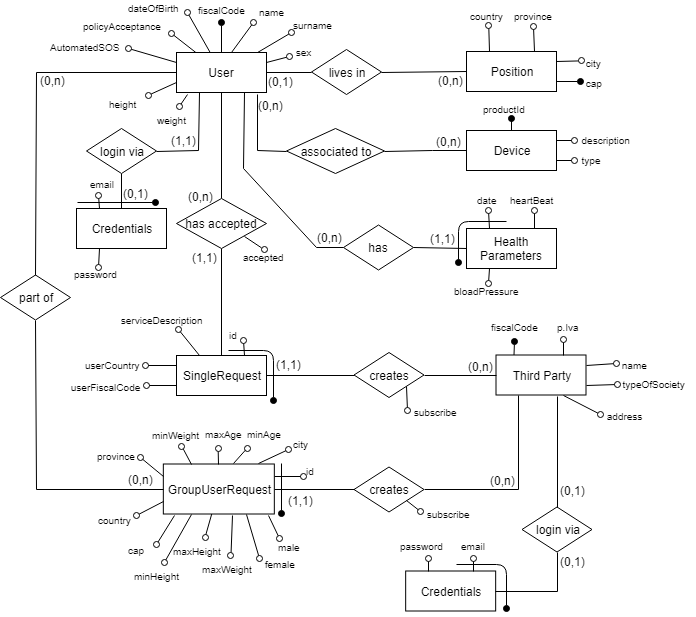
\includegraphics[width=1.0\textwidth]{./pictures/ER_diagram.png}\par
	\caption{Entity Relationship diagram}
\end{figure}
\FloatBarrier
